\documentclass{article}
\usepackage[T1]{fontenc}
\usepackage{lmodern}
\usepackage{graphicx}
\usepackage{amsmath,amssymb}
\usepackage[a4paper,margin=2cm]{geometry}
\usepackage[absolute,overlay]{textpos}
\setlength{\TPHorizModule}{1mm}
\setlength{\TPVertModule}{1mm}
\usepackage[indonesian]{babel}
\usepackage{hyperref}
\setlength{\emergencystretch}{2em}
% unit: Halaman 7

\begin{document}

% === Halaman 7 (llm) ===

% (tidak ada teks dari model)

% deskripsi: Diagram alur proses enkripsi menggunakan jaringan Feistel 16-round, yang menunjukkan input plaintext P (64 bits), proses Initial Permutation (IP), ekspansi kunci K menjadi K1 sampai K16, proses Enciphering, Inverse Initial Permutation (IP-1), dan output ciphertext C (64 bits).
% bbox normalisasi: [0.0500, 0.0800, 0.9300, 0.8300]
\begin{textblock*}{184.80mm}(10.50mm,23.76mm)
\noindent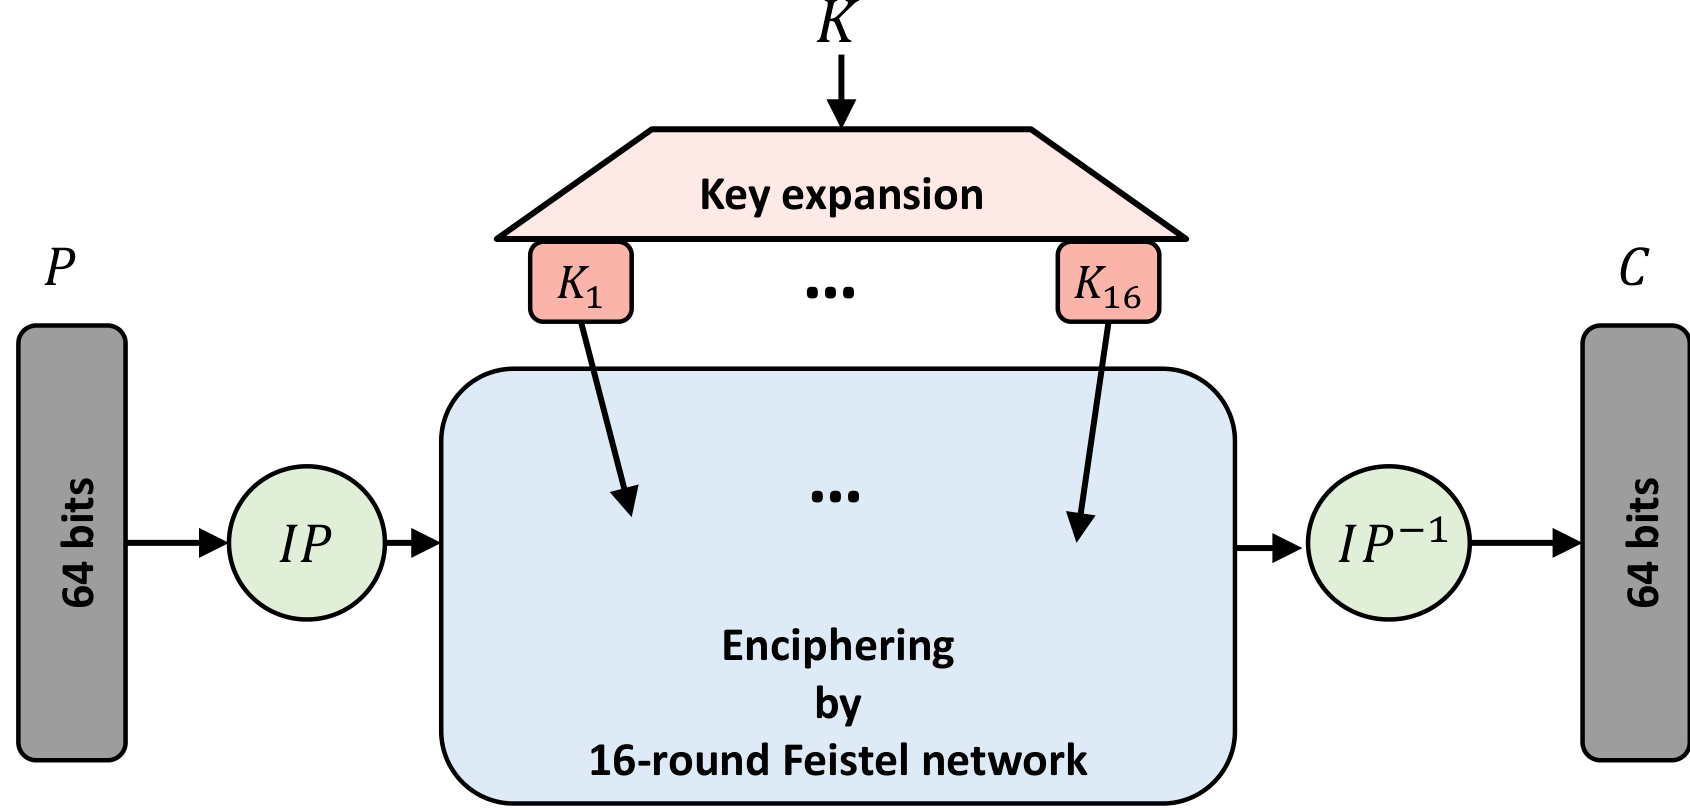
\includegraphics[width=184.80mm,height=222.75mm]{../../images/llm/page_007_img_01.png}%
\end{textblock*}

\end{document}
